\documentclass[utf8]{ctexart}
\usepackage{mathtools}
\usepackage{amsmath}
\usepackage{graphicx}
\title{\zihao{1}作业22}
\author{\zihao{-3}CarBO}
\date{}
\begin{document}
\maketitle
    \section{有$v_0$,$v_1$是两个四元数,其夹角为$\theta$。假设在它们中间进行四元数插值结果为$v^\prime$,
    $v^\prime$和$v_1$之间夹角为$\theta^\prime<\theta$,记$v_\perp$是垂直于$v_1$的四元数向量,证明:
    $v^\prime=v_1\cos\theta^\prime+v_\perp\sin\theta^\prime$}
    \begin{figure}[h]
        \centering
        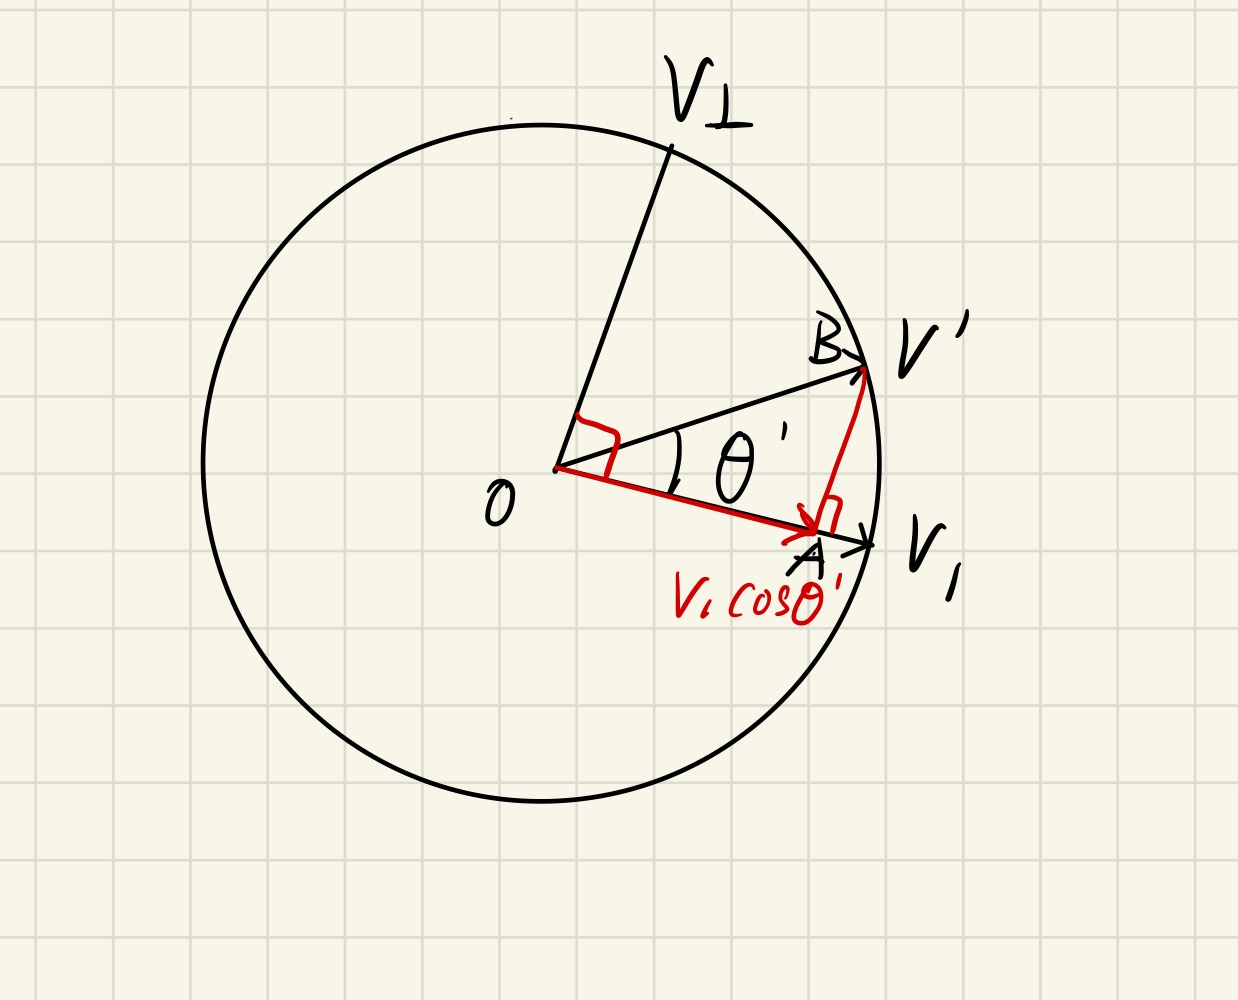
\includegraphics[scale=0.6,width=8cm,height=6cm]{1111.jpg}
    \end{figure}
    由图和单位四元数可知,$v_\perp$与AB平行,有 $\overrightarrow{AB}$方向与$v_\perp$同向,

    $\|\overrightarrow{AB}\| =\|v^\prime\cdot\sin\theta^\prime\|=\|\sin\theta^\prime\|$,
    因此$\overrightarrow{AB} =v_\perp\cdot\sin\theta^\prime$


    因为$v^\prime$与$v_1$大小相等,有
    $\|\overrightarrow{OA}\|=\|v^\prime\cdot\cos\theta^\prime\|=\|\cos\theta^\prime\|$

    方向与$v_1$同向,因此$\overrightarrow{OA}=v_1\cdot\cos\theta^\prime$


    故$\overrightarrow{OB}=\overrightarrow{OA}+\overrightarrow{AB}
    =v_\perp\cdot\sin\theta^\prime+v_1\cdot\cos\theta^\prime$
\end{document}